\section{Effects and handlers}
\begin{frame}
  \frametitle{Effects and handlers}
  \begin{definition}[Algebraic effect]
    An effect is a collection of abstract operations, e.g. 
    $\{ Op_i : a_i \to b_i \}$
  \end{definition}
  \begin{definition}[Effect handler]
    An effect handler interprets operations.
  \end{definition}
  \begin{block}{Computations as trees}
    Intuitively, we can think of operations as \emph{nodes} in computation trees, and handlers as computation tree transformers \cite{Lindley14}.
  \end{block}
  % \begin{block}{Alternative interpretation through duality}
  %   Conceptually, operations and handlers are dual \cite{Plotkin13}:
  %   \begin{itemize}
  %     \item Operations are \emph{effect constructors}.
  %     \item Handlers are \emph{effect destructors}.
  %   \end{itemize}
  % \end{block}
\end{frame}

% \begin{frame}
%   \frametitle{Modularity}
%   \begin{block}{Modular abstraction}
%     Operations are abstract and compose seamlessly.
%   \end{block}
%   \begin{block}{Modular instantiation}
%     Handlers interprets operations concretely.
%   \end{block}
%   Thus, an operation can have multiple different interpretations.
% \end{frame}

\begin{frame}[fragile]
  \frametitle{Design}
  \begin{block}{Handlers}
    Essentially, handlers embody a collection of case-statements, e.g.
\begin{lstlisting}[basicstyle=\ttfamily]
handle(x) {
  case Op1(p,k)  -> ...
  case OpN(p,k)  -> ...
  case Return(x) -> ...
} 
\end{lstlisting}
This style is adapted from Plotkin and Pretnar \cite{Plotkin13,Kammar13}.
  \end{block}
  \begin{block}{Operation discharge}
    Operations are discharged using the ``do'' primitive, e.g.
    \texttt{do Op(arg)}
  \end{block}
\end{frame}

\begin{frame}[label={choice}]
  \frametitle{Make a choice!}
  \begin{center}    
    \begin{figure}
      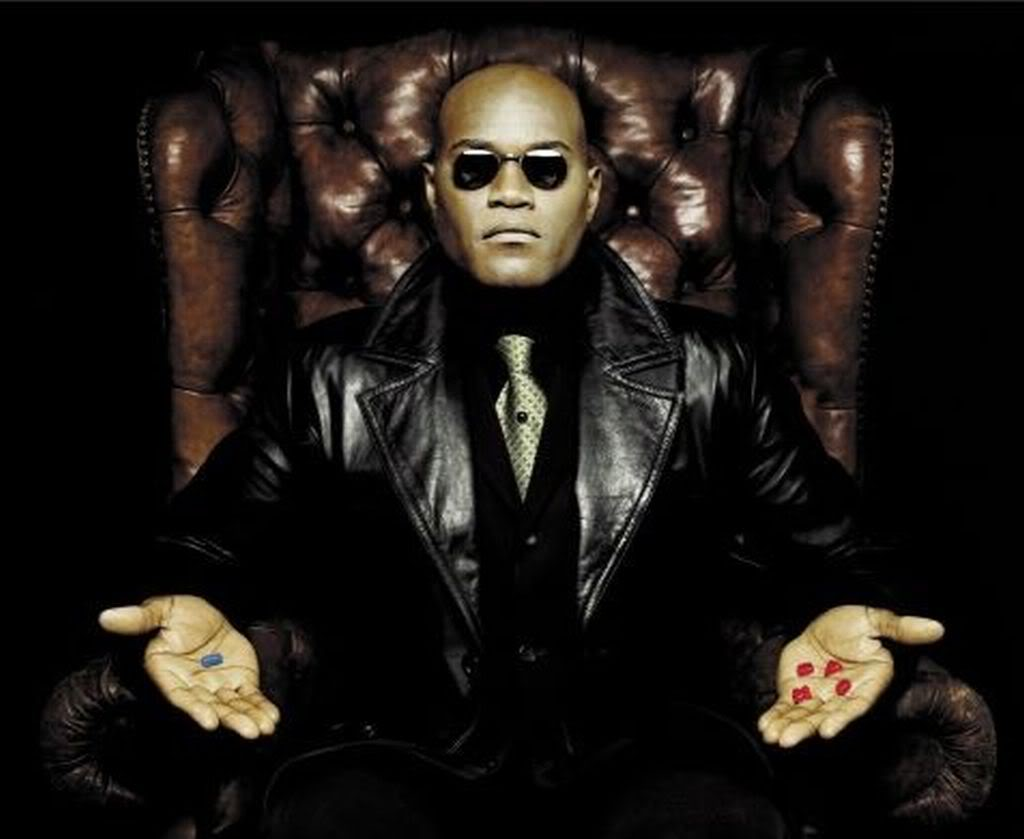
\includegraphics[scale=0.2]{choice.jpg}
    \end{figure}
    Live demo or \hyperlink{backup}{backup slides}?
  \end{center}
\end{frame}

\begin{frame}
  \frametitle{How does row polymorphism fit into this?}
  \begin{itemize}
    \item Handlers get typed as
  \[ \texttt{fun} : (() \xrightarrow{\{Op_1:a_1 \to b_1,\dots,Op_n:a_n \to b_n \}\;} c) \to c \]
  that is, they are closed.\\
\item \uncover<2->{We want \emph{open} handlers too, e.g.}
  \uncover<2->{\[ \texttt{fun} : (() \xrightarrow{\{Op_1:a_1 \to b_1,\dots,Op_n:a_n \to b_n \; | \; \rho \}\;} c) \to c \]
Consequently, we obtain a high-degree of modularity.
}

\end{itemize}
\end{frame}

\begin{frame}
  \frametitle{Wrap up}  
  At this stage
  \begin{itemize}
    \item Front end stuff.
    \item Added user-defined effects.
    \item Type checking handlers and operations.
    \item Almost done implementing closed handlers.
  \end{itemize}
  Todo in the near future
  \begin{itemize}
    \item Add open handlers.
    \item Programming with handlers and effects.
    \item Explore generalisations.
    \item Refactor.
    \item Write-up.
  \end{itemize}
\end{frame}